\chapter{Una hora escrita con Sol -- I}

\lettrine[ante=\raisebox{-1.5ex}{\large ---},lines=2]{M}{uy bien,
  Antonia} ---comenzó Cecilia con en\-tu\-sias\-mo---. Ya sabemos cómo
formar cada dígito y cómo calcular el ángulo con que cada uno de ellos
debe cortar el cuerpo del reloj; ahora sólo debemos, para cada hora
del día, agrupar los dígitos correspondientes y... ¡ya tenemos reloj
de Sol digital!

Cecilia miró a Antonia con una sonrisa radiante, pero encontró en su
amiga una expresión taciturna:

---Antonia... ¿pasa algo?  ---preguntó.

Antonia pareció salir lentamente de su ensimismamiento:

---No, no... para nada ---contestó, pero sus manos se mantenían,
contrariamente a su costumbre, lejos del teclado.

---Pues no parece ---objetó su amiga, frunciendo el ceño---.  Ya casi
logramos nuestro objetivo... ¿no te pone contenta?

---Bueno... sí, sí, claro ---admitió Antonia sin mucha convicción,
mientras se incorporaba con cierto esfuerzo en la silla como quien
trata de afirmar sus dichos con la postura corporal.

Cecilia adivinó de pronto lo que estaba sucediendo; suavemente
preguntó:

---¿No te gusta la idea de terminar el reloj, no?

Antonia sonrió con tristeza, y con un gesto de alivio al verse
sorprendida en su paradójica melancolía, suspiró:

---Supongo que soy bastante predecible... Bien, sí: para qué te lo voy
negar: estamos a punto de terminar el reloj, y ya estoy extrañando
estas reuniones.

Cecilia sonrió con ternura:

---Vamos, Antonia; te conozco: ¡Ya se te va a ocurrir otra cosa tanto
o más loca que este reloj! ---y ambas rieron con ganas.

Antonia finalmente tomó el teclado con decisión:

---Bien, necesitamos un módulo que reciba la hora que queremos
producir. No hace falta pasarle ningún ángulo: el mismo depende
precisamente de la hora, así que será calculado por el mismo módulo.

\begin{lstlisting}
module hora_solar(hora){

}
\end{lstlisting}


%       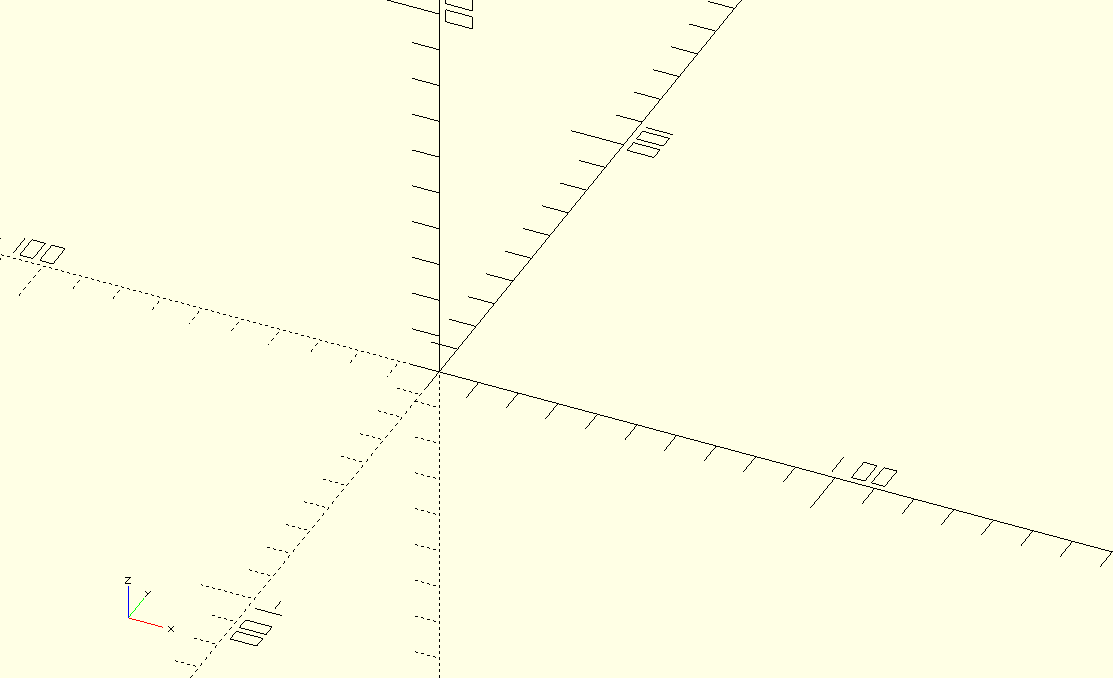
\includegraphics[width=2cm]{vacio}

Antonia se reclinó contra la silla, mirando el texto con la cabeza
ligeramente ladeada:

---Hmmm... esto nos permitirá pedir algo tan natural como
\lstinline!hora_solar(12)!, pero ¿cómo hacemos con las 12:30, por
ejemplo? No sé si me gusta tanto la expresión
\lstinline!hora_solar(12.5)!... Por otra parte, \lstinline!12:30!
claramente no es un número. Creo que lo mejor es pasar al módulo la
hora y los minutos por separado.

\begin{lstlisting}
module hora_solar(horas,minutos){

}
\end{lstlisting}

%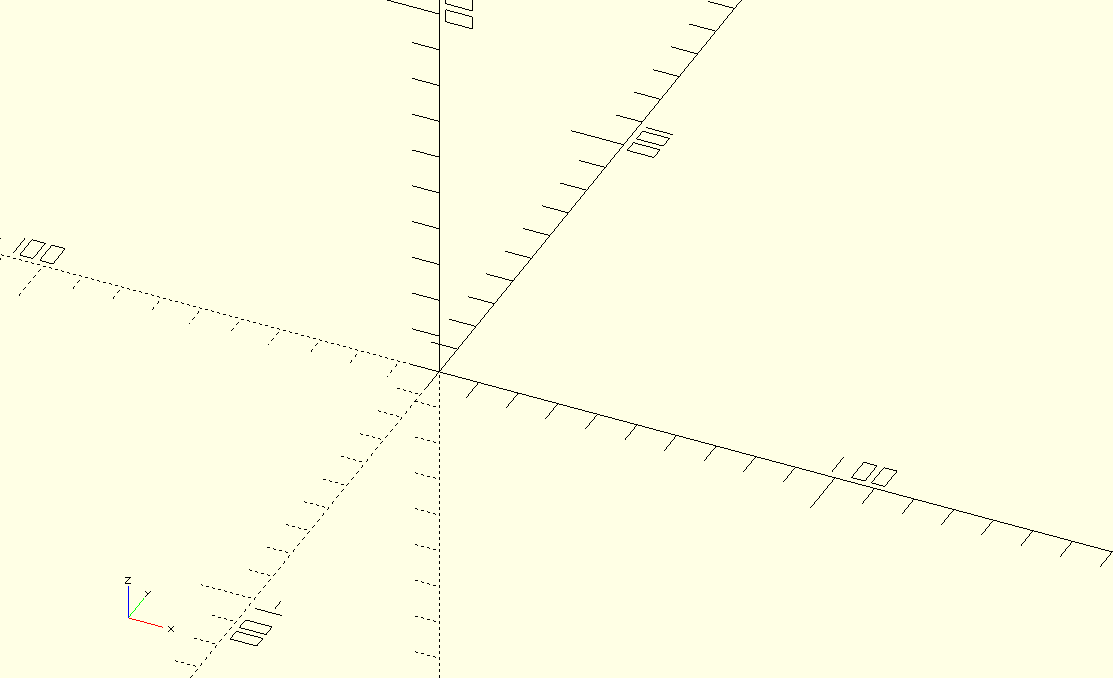
\includegraphics[width=2cm]{vacio}

Cecilia no estaba muy segura de la superioridad de la segunda versión;
pero tampoco le parecía peor, así que decidió confiar en la intuición
de su amiga.

---Ahora debemos calcular el ángulo correspondiente; nada más fácil
---aseguró Antonia, con evidente satisfacción.

\begin{lstlisting}
module hora_solar(horas,minutos){
  alfa=alfa(horas+minutos/60);
}
\end{lstlisting}

%       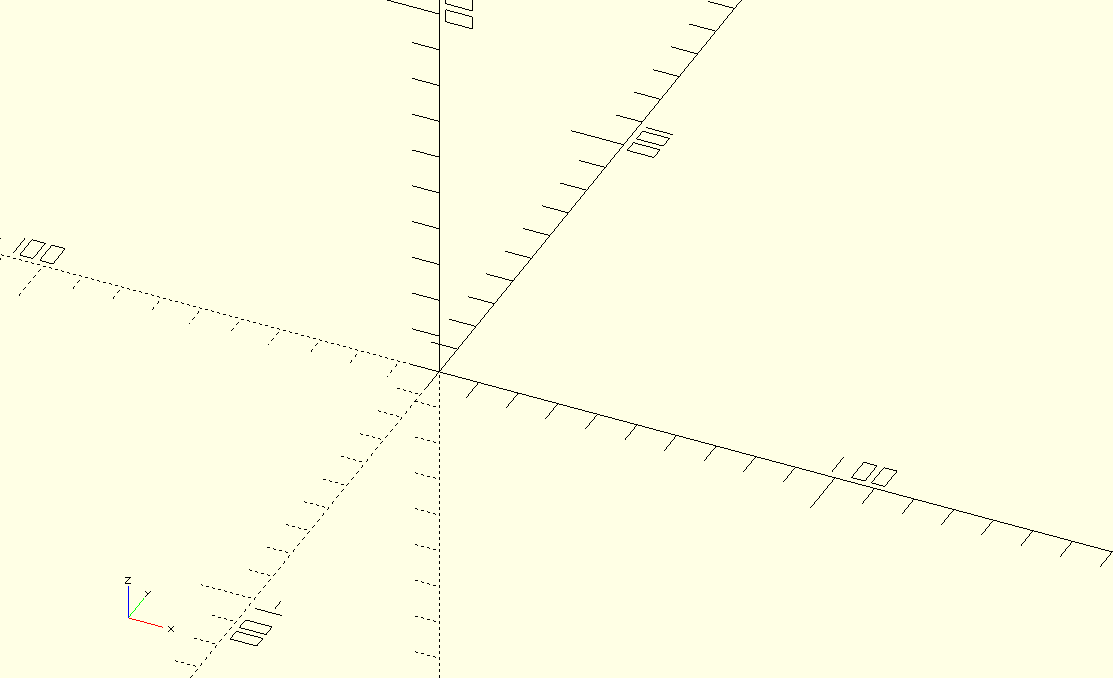
\includegraphics[width=2cm]{vacio}


Cecilia sonrió, divertida: la función \lstinline!alfa! requería la
hora en unidades de horas: nada más simple de conseguir, simplemente
sumando los \lstinline!minutos! divididos por 60 a las
\lstinline!horas!.

---Ahora viene la parte más difícil ---advirtió Antonia---: debemos
obtener los dígitos que forman las horas y los minutos. Por ejemplo,
si el módulo es invocado como \lstinline!hora_solar(12, 30)!, de
alguna forma debe poder obtener un `1', un `2', un `3' y un
`0'. Convendría almacenar cada dígito en una variable.
 

\begin{lstlisting}
module hora_solar(horas,minutos){
  alfa=alfa(horas+minutos/60);
  hora_decenas= ? ;
  hora_unidades= ? ;
  minuto_decenas= ? ;
  minuto_unidades= ? ;
}
\end{lstlisting}

%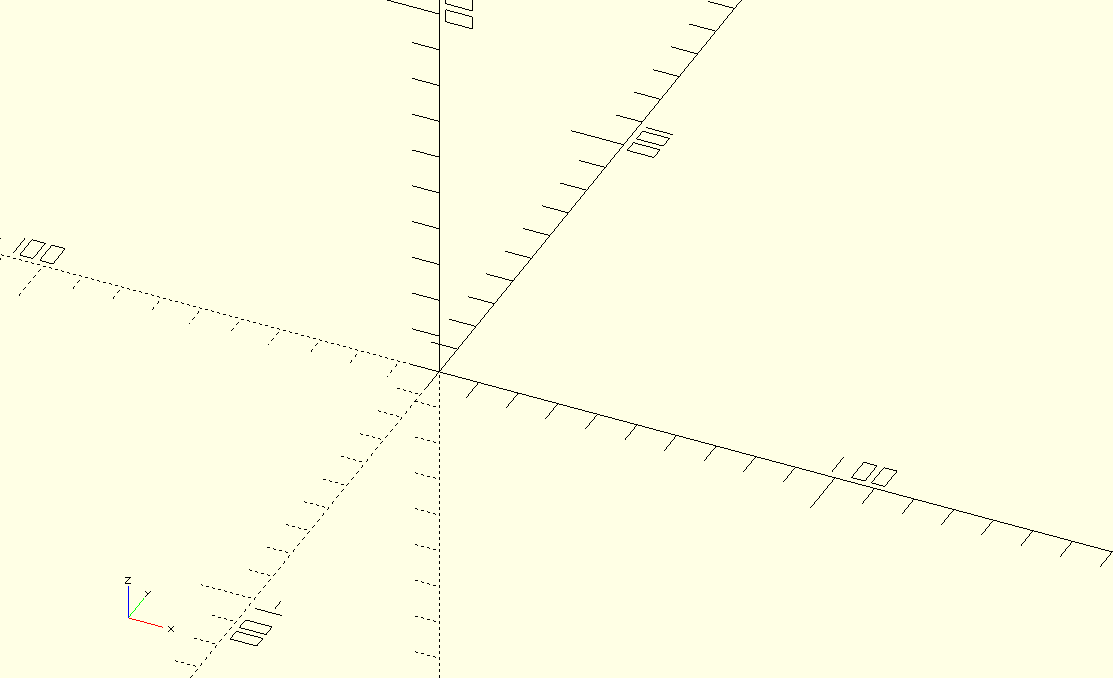
\includegraphics[width=2cm]{vacio}

Cecilia sintió que podían evitarse un problema:

---¿Y no podemos sencillamente enviar al módulo cada dígito? Quiero
decir, reescribirlo así:

\begin{lstlisting}
module hora_solar(hora_decenas, hora_unidades, minuto_decenas, minuto_unidades){

}  
\end{lstlisting}


Cecilia no había terminado su sugerencia cuando el gesto de su amiga
hizo que se arrepintiera.

---¡Ay, Cecilia!  ---Antonia no disimuló su expresión de
de\-sa\-gra\-do---. ¡Qué definición tan fea!  No me imagino pidiendo,
ni siquiera a un módulo, que me muestre la hora 1, 2, 3, 0...

---¿La hora 12, 30 te parece mucho mejor? ---replicó Cecilia, algo
mortificada.

Antonia no pareció captar la mordacidad del comentario de Cecilia:

---Sinceramente, sí: puedo imaginarme invocando este módulo con un
bucle que recorra las horas, de 6 a 18, y para cada una de ellas los
minutos, de 0 a 59. Pero ya llegaremos a eso ---Antonia parecía ahora
apurada por continuar---. Veamos cómo rescatar dígitos de un número;
creo que es tarea para una nueva función.

\section{Función resto}
                                
---Vamos a necesitar la función que calcula el resto de un cociente
---adelantó Antonia.

\begin{lstlisting}[numbers=none]
echo(18%2,19%2,21%3,23%3);
\end{lstlisting}

\begin{figure}[ht]
  \centering
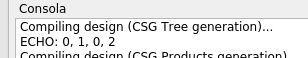
\includegraphics[width=.75\textwidth]{imagenes/restos-2-y-3}  
  \caption{Función resto.}
  \label{fig:restos-2-y-3}
\end{figure}


\guillemotright \lstinline!n%m! devuelve el resto del cociente
$\frac{n}{m}$; de esta forma, \lstinline!18%2=0!, ya que 18 es un
número par, mientras que \lstinline!19%2=1!. De la misma manera,
\lstinline!21%3=0! y \lstinline!23%3=2!.

---¡Bien! Ahora ya sabemos distinguir los números pares de los
impares ---Cecilia seguía un poco molesta, y lo expresaba con ironías no
demasiado sutiles. Antonia, según su costumbre, no dio muestras de
percibirlo y continuó:

---Nosotras, en nuestro reloj, podemos aprovechar esta función para
rescatar dígitos:

\begin{lstlisting}[numbers=none]
echo(1%10, 12%10, 123%10, -1234%10);
\end{lstlisting}

\begin{figure}[ht]
  \centering
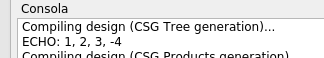
\includegraphics[width=.75\textwidth]{imagenes/resto-10}  
\caption{El resto de la división por 10 rescata las unidades de un
  número, incluido el signo.}
  \label{fig:resto-10}
\end{figure}


Cecilia no pudo evitar que un súbito entusiasmo le cambiara el gesto:
apreció claramente que el resto de un número dividido por 10 le
devolvía las unidades del mismo... ¡incluyendo su signo!

Antonia sonrió al comprobar el efecto que la aplicación de la nueva
función produjo en Cecilia:

---Bien, ya sabemos cómo rescatar las unidades... ¿Cómo hacemos ahora
con las decenas? Y, ya que estamos, con cualquier otra posición: sería
una pena no escribir una función bien general, que merezca la
aprobación hasta del exigente editor de este
manualcito.\footnote{¡Hey! No me hagan \emph{bullying}. (Nota del
  Editor)}$^,$\footnote{Disculpá; era una broma. (Nota de Antonia)}
Pienso en algo como una función \lstinline!n_a_digito(n,p)!, donde
\lstinline!n! es el número a diseccionar y \lstinline!p! la posición
del dígito que queremos obtener, contando desde las unidades; por
ejemplo, que \lstinline!n_a_digito(-1837,0)! diera -7 y
\lstinline!n_a_digito(1986,2)! devolviera 9.

Cecilia encontró el desafío muy estimulante; probó un poco al azar:

---¿Y si hacemos \lstinline!n%100! no obtendremos las decenas...?
---dijo, mientras tomaba el teclado para sí.


\begin{lstlisting}[numbers=none]
echo(1971%100);
\end{lstlisting}

\begin{figure}[ht]
  \centering
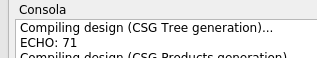
\includegraphics[width=.75\textwidth]{imagenes/resto-100}  
\caption{El resto de la división por 100 devuelve las decenas
  \emph{completas} de un número.}
  \label{fig:resto-100}
\end{figure}


Cecilia, ante el resultado de la figura \ref{fig:resto-100}, sintió
que sus mejillas se encendían. Antonia no encontró reparos en reírse
francamente del desliz:

---Yo hice lo mismo ---confesó---; hubiera sido muy hermoso que
funcionara. Pero el resto de dividir por 100 te devuelve \emph{todas}
las decenas, no solamente el dígito de las mismas. Así que hay que
buscar otra solución.

Cecilia se dispuso a esperar que Antonia le revelara una nueva función
mágica, pero su amiga se anticipó:

---Puede resolverse usando la función `resto' ---y no dijo más.

Cecilia se sintió tocada en su amor propio; concentró su mirada en el
monitor. <<Muy bien>> ---pensó---, <<si hago \lstinline!n%10! obtengo
las unidades de \lstinline!n!. Yo quiero el dígito que corresponde a
las decenas. ¡Ay!, si solamente ese dígito ocupara el lugar de las
unidades, podría rescatarlo como una unidad más...>>.

Cecilia frunció el ceño para obligarse a pensar, y cruzó sus brazos
contra el pecho; su vista ya se perdía más allá del monitor de la
computadora. De pronto y una vez más la epifanía ocurrió:

---¡Claro! ---dijo en voz alta, sin darse cuenta---.  ¡Puedo llevar
las decenas al lugar de las unidades!  ¡Simplemente debo dividir
previamente el número por 10! ---y sus dedos volaron sobre el teclado.

\begin{lstlisting}[numbers=none]
echo( (1971/10)%10 );
\end{lstlisting}

\begin{figure}[ht]
  \centering
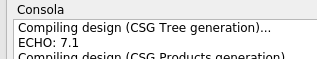
\includegraphics[width=.75\textwidth]{imagenes/resto-decenas-1}  
\caption{Primer intento (fallido) de Cecilia para rescatar el dígito
  de las decenas.}
  \label{fig:resto-decenas-1}
\end{figure}


Un gesto de desazón cubrió el rostro de Cecilia mientras se
desplomaba contra el respaldo de su silla.

---Corriste \emph{todo} el número hacia la derecha, y eso incluía a
las unidades, que ahora aparecen como un decimal ---Antonia confirmó
el diagnóstico que Cecilia podía ver por sí misma claramente---. La
idea está bien; sólo debemos deshacernos de ese molesto decimal.

\section{Funciones de redondeo y truncamiento}

---Para aliviar a un número de decimales resultan muy útiles las
  funciones \lstinline!round!, \lstinline!floor! y
  \lstinline!ceil! ---explicó Antonia---. La primera
  redondea al número entero más cercano.

\begin{lstlisting}[numbers=none]
echo(round(3.14), round(2.72), round(-3.14), round(-2.72));
\end{lstlisting}

\begin{figure}[ht]
  \centering
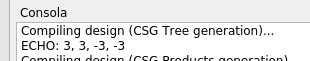
\includegraphics[width=.75\textwidth]{imagenes/round}  
  \caption{Función \lstinline!round!.}
  \label{fig:round}
\end{figure}


\guillemotright \lstinline!floor! te redondea `para abajo'.

\begin{lstlisting}[numbers=none]
echo(floor(3.14), floor(2.72), floor(-3.14), floor(-2.72));
\end{lstlisting}

\begin{figure}[ht]
  \centering
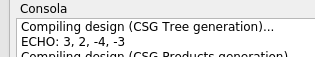
\includegraphics[width=.75\textwidth]{imagenes/floor}  
  \caption{Función \lstinline!floor!.}
  \label{fig:floor}
\end{figure}

\guillemotright Por su parte, \lstinline!ceil! redondea `hacia arriba'.

\begin{lstlisting}[numbers=none]
echo(ceil(3.14), ceil(2.72), ceil(-3.14), ceil(-2.72));
\end{lstlisting}

\begin{figure}[ht]
  \centering
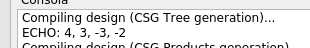
\includegraphics[width=.75\textwidth]{imagenes/ceil}  
  \caption{Función \lstinline!ceil!.}
  \label{fig:ceil}
\end{figure}

Cecilia sintió que recobraba el entusiasmo; recorrió las tres
funciones para decidir con cuál aligerar su propia función de los
indeseables decimales, pero tras unos instantes se sintió confundida:
ninguna parecía cumplir con sus deseos. Necesitaba una función que
siempre podara los decimales; algo que tomara los valores 3.14, 2.72,
-3.14 y -2.72 y devolviera 3, 2, -3 y -2, respectivamente. Cuando
giró, perpleja, en dirección a Antonia, la encontró sonriendo, como si
hubiera adivinado sus pensamientos:

---Como ya sin duda descubriste, ninguna de esas funciones basta para
resolver por sí sola nuestro problema. La función que necesitamos es
una que trunque un número sin miramientos ---con\-fir\-mó
Antonia---. Pero, curiosamente, esa función en \openscad{} no
existe..: ¡Mejor! ---agregó, con una sonrisa exultante---. Así la
creamos nosotras. En todos los lenguajes de programación que conozco
esa función se denomina \texttt{truncate}; podemos usar ese mismo
nombre, si te parece.

Cecilia no se sentía con ganas de discutirlo: sólo quería seguir con
el módulo \lstinline!hora_solar!, que tan lejos había quedado.

Antonia, ante el mutismo de Cecilia, le señaló con el mentón el
teclado. Ésta, con un suspiro de resignación, lo tomó dispuesta a
escribir una nueva función que supliera la curiosa omisión del
lenguaje de \openscad{}. Pero antes, se permitió una queja: 

---Antonia, me dijiste hace unos momentos que sólo era necesaria la
función resto, y ahora resulta que también hace falta una inexistente
función de truncamiento...

---Soy docente ---replicó Antonia, con gesto burlón---: ¿cuándo
aceptarás que no podés creer en todo lo que digo?

Cecilia tampoco quiso discutir esto; volvió su mirada al monitor y
enfocóse en el nuevo problema que tenía delante.

<<Muy bien, Cecilia>> ---pensó---. <<La función \lstinline!floor!
parece funcionar para números positivos, mientras que \lstinline!ceil!
es apropiada para los negativos. Si pudiera decidir, dentro de la
función, qué tipo de redondeo aplicar dependiendo del signo del número
recibido...>> ---no pasó mucho tiempo hasta que se le ocurrió probar
con el operador ternario `\lstinline!? :!'.

\begin{lstlisting}
function truncate(n)=
  n<0 ? ceil(n) : floor(n);

echo(truncate(3.14), truncate(2.72), truncate(-3.14), truncate(-2.72));
\end{lstlisting}

\begin{figure}[ht]
  \centering 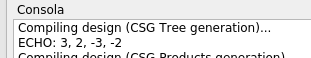
\includegraphics[width=.6\textwidth]{imagenes/truncate-1}
  \caption[Función \lstinline!truncate!]{Cecilia crea la función
    \lstinline!truncate!.}
  \label{fig:truncate-1}
\end{figure}


Cecilia estuvo a punto de saltar de su silla: el código no sólo
funcionaba, sino también le parecía muy hermoso. La nueva función
\lstinline!truncate!  se fijaba si el número recibido era menor que 0:
en ese caso, devolvía \lstinline!ceil(n)!; en caso contrario,
\lstinline!floor(n)!.

Antonia aplaudió lentamente, con gesto de feliz ad\-mi\-ra\-ción:

---Excelente, Cecilia, pero no cantemos victoria: ¿funciona con 0?
Siempre hay que probar los valores críticos...

Cecilia sintió que un nudo le apretaba la garganta; con un vago temor,
hizo la prueba.

\begin{lstlisting}
echo(truncate(0));
\end{lstlisting}

\begin{figure}[ht]
  \centering
  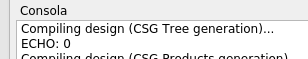
\includegraphics[width=.6\textwidth]{imagenes/truncate-0}
  \caption{Cecilia verifica cándidamente que
    \lstinline!truncate(0)=0!.}
  \label{fig:truncate-0}
\end{figure}
  

Mientras Antonia reía alegre y francamente, Cecilia no pudo menos que
sonreír al advertir la trampa inocente en la que había caído:
cualquiera de las dos funciones hubiera servido con 0.

---Bueno, Cecilia; creo que ahora podemos obtener las decenas de
cualquier número, ¿no? ---preguntó retóricamente Antonia.

Cecilia estaba de acuerdo de todo corazón.

\begin{lstlisting}[numbers=none]
echo( truncate(1971/10)%10, truncate(-753/10)%10 );
\end{lstlisting}

\begin{figure}[ht]
  \centering
  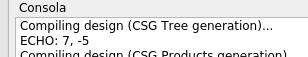
\includegraphics[width=.6\textwidth]{imagenes/decenas-bien}
  \caption{Cecilia comprueba que puede obtener las decenas de
    cualquier número.}
  \label{fig:decenas-bien}
\end{figure}
  

Antes de que interviniera Antonia, Cecilia añadió:

---Y si queremos obtener las centenas, la manera es evidente.

\begin{lstlisting}[numbers=none]
echo( truncate(2021/100)%10, truncate(-480/100)%10 );
\end{lstlisting}

\begin{figure}[ht]
  \centering
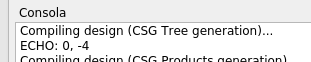
\includegraphics[width=.6\textwidth]{imagenes/centenas}  
  \caption{Obtención de las centenas.}
  \label{fig:centenas}
\end{figure}


---Perfecto ---confirmó Antonia, tomando ahora el te\-cla\-do---.  Pasemos
en limpio, entonces:

\begin{tabular}{lr}
    Para las unidades:    & \lstinline!truncate(n/1)%10! \\
    Para las decenas:    & \lstinline!truncate(n/10)%10! \\
    Para las centenas:    & \lstinline!truncate(n/100)%10! \\
    Etc...
\end{tabular}
  
---¿Por qué dividiste \texttt{n} por 1 para las unidades?
---pre\-gun\-tó Cecilia con visible extrañeza.

---Para hacer evidente el patrón que necesitamos aprehender a fin de
escribir la función \lstinline!n_a_digito! de manera general
---jus\-ti\-fi\-có Antonia.

Cecilia lo encontró razonable; supuso que el empleo de
\texttt{truncate} también para las unidades tenía la misma
explicación. Sin que Antonia se lo sugiriera, tomó el teclado mientras
pensaba: <<La función que voy a escribir recibirá dos parámetros:
\texttt{n} y \texttt{p}. El primero es el número a analizar y el otro
es el dígito que quiero rescatar, de manera que \lstinline!p=0! indica
las unidades, \lstinline!p=1! las decenas, etc.>> Con la mirada fija
en la tabla escrita por Antonia, siguió sumida en sus
pensamientos---. <<La fórmula es la misma para todos las posiciones,
salvo por el valor que divide a \texttt{n} antes del truncamiento: 1
cuando \lstinline!p=0!, 10 cuando \lstinline!p=1!, 100 para
\lstinline!p=2!... Son todas potencias de 10...>>, y la epifanía
volvió a ocurrir, ya por tercera vez en el capítulo:

---¡Claro! ¡El divisor de \texttt{n} es igual a $10^p$ en todos los
casos! ---afirmó Cecilia ahora en voz alta, y sin esperar la
confirmación de Antonia se lanzó a escribir la función.

\begin{lstlisting}
// p es la posicion del digito a obtener: 
// 0 para las unidades, 1 para las decenas, etc.
function n_a_digito(n,p)= 
  truncate(n/pow(10,p))%10;

echo(n_a_digito(1971,0), n_a_digito(-1986,1), n_a_digito(2021,2));
\end{lstlisting}

\begin{figure}[ht]
  \centering
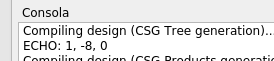
\includegraphics[width=.6\textwidth]{imagenes/n-a-digito-1}  
\caption[Función \lstinline!n_a_digito!.]{Función que rescata un
  dígito de un número.}
  \label{fig:n-a-digito-1}
\end{figure}


Cecilia, una vez más, estuvo a punto de gritar de alegría. Miró a
Antonia con gesto radiante, y encontró en el rostro de su amiga el
reflejo de su propia felicidad. Sin embargo, tras unos instantes, Antonia sumó
a su sonrisa una sombra de malicia:

---Cecilia, ¿no sería lindo que nuestra función fuera capaz de
extraer, además, los dígitos que forman los decimales de un número?
Quiero decir que, por ejemplo, haciendo \lstinline!n_a_digito (3.1416, -1)!  obtuviéramos 1.

Cecilia pensó que quizá lo sería, pero a esta altura no tenía tantas
ganas de meter mano en su hermosa y flamante función. Además, no
parecía que fuera necesaria esa funcionalidad extra para manipular las
horas del reloj, que sólo serían valores enteros.

Con la sonrisa aún más marcada, Antonia preguntó con inocencia:

---¿Me dejás probar..?

Cecilia, de puro educada, le cedió sin entusiasmo y algo de aprensión
el teclado. Pero Antonia no modificó en nada su función; tan sólo
escribió:

\begin{lstlisting}[numbers=none]
echo(n_a_digito(3.1416,-1), n_a_digito(-3.1416,-2));
\end{lstlisting}

\begin{figure}[ht]
  \centering
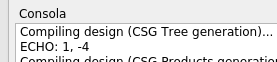
\includegraphics[width=.6\textwidth]{imagenes/n-a-digito-2}  
\caption[Dígitos decimales.]{La función \lstinline!n_a_digito!  es
  capaz de devolver también dígitos decimales.}
  \label{fig:n-a-digito-2}
\end{figure}


Tras un instante de perplejo silencio, Cecilia cubrió sus ojos con una
mano, mientras Antonia volvía a reír con ganas. <<¡Por supuesto!>>
---pensó Cecilia--- <<Caí otra vez: el código ya abarca todos los dígitos
posibles, puesto que dividir por $10^{-2}$, por ejemplo, es lo mismo
que multiplicar por $10^2$, lo cual no hace más que llevar el segundo
decimal al lugar `mágico' de las unidades>>.

Cuando Antonia dejó de reír encontró a Cecilia con ganas de continuar.

---Bien ---dijo ésta, recuperando el teclado---; creo que ya podemos
empezar a completar nuestro ya casi olvidado módulo
\lstinline!hora_solar!, ¿no te parece?


\begin{lstlisting}
module hora_solar(horas,minutos){
  alfa=alfa(horas+minutos/60);
  hora_decenas=n_a_digito(horas,1);
  hora_unidades=n_a_digito(horas,0);
  minuto_decenas=n_a_digito(minutos,1);
  minuto_unidades=n_a_digito(minutos,0);

  echo(hora_decenas, hora_unidades, minuto_decenas, minuto_unidades);
 }
\end{lstlisting}

\guillemotright La línea 8 la añadí sólo para comprobar que todo
funciona como es debido ---aclaró Cecilia---. ¿A ver si es así..?

\begin{lstlisting}[numbers=none]
hora_solar(12,30);
\end{lstlisting}

\begin{figure}[ht]
  \centering
  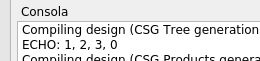
\includegraphics[width=.6\textwidth]{imagenes/hora-prueba-1}
  \caption[Dígitos de la hora.]{Cecilia comprueba que la función
    \lstinline!hora_solar! consigue los dígitos de la hora y los
    minutos.}
  \label{fig:hora-prueba-1}
\end{figure}
  

Parecía que sí.



%%% Local Variables:
%%% mode: latex
%%% TeX-master: "../libro"
%%% End:
